\documentclass{report}
\usepackage{graphicx, tikz-cd, float, titlepic, booktabs} % Required for inserting images
\usepackage{pgfplots}
\usepackage{multicol}
\usepackage{makecell}
\pgfplotsset{compat=1.15}
\usepackage{mathrsfs}
\usetikzlibrary{arrows}
\usepackage{amsmath, amssymb, amsthm, amsfonts, siunitx, physics, gensymb}
\AtBeginDocument{\RenewCommandCopy\qty\SI}
\usepackage[version=4]{mhchem}
\usepackage[most,many,breakable]{tcolorbox}
\usepackage{xcolor, fancyhdr, varwidth}
\usepackage[Glenn]{fncychap}
%Options: Sonny, Lenny, Glenn, Conny, Rejne, Bjarne, Bjornstrup
\usepackage{hyperref, cleveref}
\usepackage{icomma, enumitem} %comma as decimal and continue enumerate with [resume]
\usepackage{plimsoll} %use standard state symbol with \stst
\usepackage[danish]{babel}
\renewcommand{\cellalign}{cl}
\renewcommand{\theadalign}{cl}
\renewcommand\theadfont{\bfseries}
%%%%%%%%%%%%%%%%%%%%%%%%%%%%%%
% SELF MADE COLORS
%%%%%%%%%%%%%%%%%%%%%%%%%%%%%%
\definecolor{myg}{RGB}{56, 140, 70}
\definecolor{myb}{RGB}{45, 111, 177}
\definecolor{myr}{RGB}{199, 68, 64}
\definecolor{mytheorembg}{HTML}{F2F2F9}
\definecolor{mytheoremfr}{HTML}{00007B}
\definecolor{mylenmabg}{HTML}{FFFAF8}
\definecolor{mylenmafr}{HTML}{983b0f}
\definecolor{mypropbg}{HTML}{f2fbfc}
\definecolor{mypropfr}{HTML}{191971}
\definecolor{myexamplebg}{HTML}{F2FBF8}
\definecolor{myexamplefr}{HTML}{88D6D1}
\definecolor{myexampleti}{HTML}{2A7F7F}
\definecolor{mydefinitbg}{HTML}{E5E5FF}
\definecolor{mydefinitfr}{HTML}{3F3FA3}
\definecolor{notesgreen}{RGB}{0,162,0}
\definecolor{myp}{RGB}{197, 92, 212}
\definecolor{mygr}{HTML}{2C3338}
\definecolor{myred}{RGB}{127,0,0}
\definecolor{myyellow}{RGB}{169,121,69}
\definecolor{myexercisebg}{HTML}{F2FBF8}
\definecolor{myexercisefg}{HTML}{88D6D1}
%%%%%%%%%%%%%%%%%%%%%%%%%%%%%%%%%%%%%%%%%%%%%%%%%%%%%%%%%%%%%%%%%%%%%%
% Box environments for theorems and problems
%%%%%%%%%%%%%%%%%%%%%%%%%%%%%%%%%%%%%%%%%%%%%%%%%%%%%%%%%%%%%%%%%%%%%
\setlength{\parindent}{1cm}
%================================
% Question BOX
%================================
\newtcbtheorem[]{question}{Opgave}{enhanced,
	before skip=2mm,after skip=2mm, colback=red!5,colframe=red!80!black,boxrule=0.5mm,
	attach boxed title to top left={xshift=1cm,yshift*=1mm-\tcboxedtitleheight}, varwidth boxed title*=-3cm,
	boxed title style={frame code={
					\path[fill=tcbcolback]
					([yshift=-1mm,xshift=-1mm]frame.north west)
					arc[start angle=0,end angle=180,radius=1mm]
					([yshift=-1mm,xshift=1mm]frame.north east)
					arc[start angle=180,end angle=0,radius=1mm];
					\path[left color=tcbcolback!60!black!65!red,right color=tcbcolback!60!black!65!red,
						middle color=tcbcolback!80!black!65!red!1!red]
					([xshift=-2mm]frame.north west) -- ([xshift=2mm]frame.north east)
					[rounded corners=1mm]-- ([xshift=1mm,yshift=-1mm]frame.north east)
					-- (frame.south east) -- (frame.south west)
					-- ([xshift=-1mm,yshift=-1mm]frame.north west)
					[sharp corners]-- cycle;
				},interior engine=empty,
		},
	fonttitle=\bfseries,
	title={#2},#1}{def}


\makeatletter
\newtcbtheorem{Question}{Opgave}{enhanced,
	breakable,
	colback=white,
	colframe=myb!80!black,
	attach boxed title to top left={yshift*=-\tcboxedtitleheight},
	fonttitle=\bfseries,
	title={#2},
	boxed title size=title,
	boxed title style={%
			sharp corners,
			rounded corners=northwest,
			colback=tcbcolframe,
			boxrule=0pt,
		},
	underlay boxed title={%
			\path[fill=tcbcolframe] (title.south west)--(title.south east)
			to[out=0, in=180] ([xshift=5mm]title.east)--
			(title.center-|frame.east)
			[rounded corners=\kvtcb@arc] |-
			(frame.north) -| cycle;
		},
	#1
}{def}
\makeatother
%================================
% DEFINITION BOX
%================================

\newtheorem{defin}{Definition}[section] % Creates a new counter, number within section

\newtcbtheorem[number within=section, use counter*=defin]{Definition}{Definition}{enhanced,
	before skip=2mm,after skip=2mm, colback=red!5,colframe=red!80!black,boxrule=0.5mm,
	attach boxed title to top left={xshift=1cm,yshift*=1mm-\tcboxedtitleheight}, varwidth boxed title*=-3cm,
	boxed title style={frame code={
					\path[fill=tcbcolback]
					([yshift=-1mm,xshift=-1mm]frame.north west)
					arc[start angle=0,end angle=180,radius=1mm]
					([yshift=-1mm,xshift=1mm]frame.north east)
					arc[start angle=180,end angle=0,radius=1mm];
					\path[left color=tcbcolback!60!black,right color=tcbcolback!60!black,
						middle color=tcbcolback!80!black]
					([xshift=-2mm]frame.north west) -- ([xshift=2mm]frame.north east)
					[rounded corners=1mm]-- ([xshift=1mm,yshift=-1mm]frame.north east)
					-- (frame.south east) -- (frame.south west)
					-- ([xshift=-1mm,yshift=-1mm]frame.north west)
					[sharp corners]-- cycle;
				},interior engine=empty,
		},
	fonttitle=\bfseries,
	title={#2},#1}{def}

\newtcbtheorem[number within=section]{definition}{Definition}
{%
	enhanced,
	breakable,
	colback = red!5,
	frame hidden,
	boxrule = 0sp,
	borderline west = {2pt}{0pt}{solid, red!75!black},
	sharp corners,
	detach title,
	before upper = \tcbtitle\par\smallskip,
	coltitle = red!75!black,
	fonttitle = \bfseries\sffamily,
	description font = \mdseries,
	separator sign none,
	segmentation style={solid, red!75!black},
}
{th}

\newtcbtheorem{theo}%
    {Theorem}{}{theorem}
\newtcolorbox{prob}[1]{colback=red!5!white,colframe=red!50!black,fonttitle=\bfseries,title={#1}}

%================================
% NOTE BOX
%================================

\usetikzlibrary{arrows,calc,shadows.blur}
\tcbuselibrary{skins}
\newtcolorbox{note}[1][]{%
	enhanced jigsaw,
	colback=gray!20!white,%
	colframe=gray!80!black,
	size=small,
	boxrule=1pt,
	title=\textbf{Note:},
	halign title=flush center,
	coltitle=black,
	breakable,
	drop shadow=black!50!white,
	attach boxed title to top left={xshift=1cm,yshift=-\tcboxedtitleheight/2,yshifttext=-\tcboxedtitleheight/2},
	minipage boxed title=1.5cm,
	boxed title style={%
			colback=white,
			size=fbox,
			boxrule=1pt,
			boxsep=2pt,
			underlay={%
					\coordinate (dotA) at ($(interior.west) + (-0.5pt,0)$);
					\coordinate (dotB) at ($(interior.east) + (0.5pt,0)$);
					\begin{scope}
						\clip (interior.north west) rectangle ([xshift=3ex]interior.east);
						\filldraw [white, blur shadow={shadow opacity=60, shadow yshift=-.75ex}, rounded corners=2pt] (interior.north west) rectangle (interior.south east);
					\end{scope}
					\begin{scope}[gray!80!black]
						\fill (dotA) circle (2pt);
						\fill (dotB) circle (2pt);
					\end{scope}
				},
		},
	#1,
}
%================================
% EXAMPLE BOX
%================================
\newtcbtheorem[number within=section, use counter from=definition]{Example}{Example}
{%
	colback = myexamplebg
	,breakable
	,colframe = myexamplefr
	,coltitle = myexampleti
	,boxrule = 1pt
	,sharp corners
	,detach title
	,before upper=\tcbtitle\par\smallskip
	,fonttitle = \bfseries
	,description font = \mdseries
	,separator sign none
	,description delimiters parenthesis
}
{ex}
%================================
% THEOREM BOX
%================================

\tcbuselibrary{theorems,skins,hooks}
\newtcbtheorem[number within=section, use counter from=definition]{Theorem}{Theorem}
{%
	enhanced,
	breakable,
	colback = mytheorembg,
	frame hidden,
	boxrule = 0sp,
	borderline west = {2pt}{0pt}{mytheoremfr},
	sharp corners,
	detach title,
	before upper = \tcbtitle\par\smallskip,
	coltitle = mytheoremfr,
	fonttitle = \bfseries\sffamily,
	description font = \mdseries,
	separator sign none,
	segmentation style={solid, mytheoremfr},
}
{th}

%%%%%%%%%%%%%%%%%%%%%%%%%%%%%%%%%%%%%%%%%%%%%%%%%%%%%%%%%%%%%%%%%
% SELF MADE COMMANDS
%%%%%%%%%%%%%%%%%%%%%%%%%%%%%%
\newcommand{\sol}{\setlength{\parindent}{0cm}\textbf{\textit{Løsning:}}\setlength{\parindent}{1cm}}
%%%%%%%%%%%%%%%%%%%%%%%%%%%%%%%%%
\usepackage[tmargin=2cm,rmargin=1in,lmargin=1in,margin=0.85in,bmargin=2cm,footskip=.2in]{geometry}\pagestyle{fancy}
\lhead{Minrui Kevin Zhou 3.b}
\rhead{Eksamen august 2024}

\title{Eksamen august 2024\\
{\Large \textbf{3.b fysik A}}}
\author{Kevin Zhou}
\date{\today}

\begin{document}
\maketitle
\begin{question}{Minikøleskab}{}
  Et minikøleskab står tændt i 365 dage. Køleskabet omsætter elektrisk energi med effekten 47 W. 
  \begin{itemize}
    \item[a.] Beregn den elektriske energi, som minikøleskabet omsætter på 365 dage.
  \end{itemize}
  Ved en test af et minikøleskab måles temperaturen af en fyldt sodavandsdåse som funktion af tiden efter anbringelse i køleskabet. På et tidspunkt falder temperaturen med 0,46 °C pr. minut. 
  Den fyldte sodavandsdåse består af 345 g sodavand og 14,3 g aluminium. Den specifikke varmekapacitet for sodavand er 3,90 kJ/(kg$\cdot$°C).
\begin{itemize}
  \item[b.] Bestem den effekt, hvormed der afgives energi fra den fyldte sodavandsdåse, når temperaturen falder med 0,46 °C pr. minut.
\end{itemize}
\end{question}
\sol \\
\textbf{a.}
Energien, som minikøleskabet omsætter på 365 dage må være
\begin{equation*}
\begin{split}
  E &= P \cdot t \\
  &=47 \;\unit{W}  \cdot 365 \cdot 24 \cdot 60^2 \;\unit{s} \\
  &\approx 1,5 \cdot 10 ^{9} \;\unit{J} \\
  &=1,5 \;\unit{GJ}.
\end{split}
\end{equation*}
Den elektriske energi, som minikøleskabet opmsætter på 365 dage er altså $1,5 \;\unit{GJ} $. \\[1ex]
\textbf{b.}
Vi starter med at finde et udtryk for effekten.
Bemærk, at vi lader $T$ betegne temperaturen, hvor $t$ betegner tid. 
\begin{equation*}
\begin{split}
  P&=\dv{E}{t}\\
  &=-\dv{t} \left(E _{\text{alu}} + E _{\text{soda}}\right) \\
  &=-\dv{t} \left(T \cdot \left(c _{\text{alu}}\cdot m _{\text{alu}} + c _{\text{soda}} \cdot m _{\text{soda}}\right) \right) \\
  &=-\left(c _{\text{alu}}\cdot m _{\text{alu}} + c _{\text{soda}} \cdot m _{\text{soda}}\right) \cdot \dv{T}{t},
\end{split}
\end{equation*}
hvor det sidste lighedstegn gælder, da det kun er $T$, som afhænger af tiden (for både de specifikke varmekapaciter og masserne er konstante).
Det er i opgaven givet, at $\dv{T}{t}=-0,46 \;\unit{\celsius/min}$.
Vi kan nu udregne effekten $P$.
\begin{equation*}
\begin{split}
  P&=\left(c _{\text{alu}}\cdot m _{\text{alu}} + c _{\text{soda}} \cdot m _{\text{soda}}\right) \cdot \dv{T}{t}\\
  &=-\left(897 \;\unit{\frac{J}{kg \cdot \celsius}} \cdot 0,0143 \;\unit{kg} +3,90 \cdot 10^3 \;\unit{\frac{J}{kg \cdot \celsius}} \cdot 0,345 \;\unit{kg} \right) \cdot \left(-\frac{0,46}{60} \;\unit{\frac{\celsius}{s}}\right) \\
  &\approx 10 \;\unit{W}.
\end{split}
\end{equation*}
Effekten, hvormed der afgives energi fra den fyldte sodavandsdåse, når temperaturen falder med 0,46 °C pr. minut er altså $10 \;\unit{W} $.

\begin{question}{Batteribeskyttelse}{}
Spændingsfaldet over en NTC-resistor i en telefon er 4,5 V. Strømstyrken igennem NTC-resistoren må højst være 0,21 mA.
\begin{itemize}
  \item[a.] Beregn den afsatte effekt i NTC-resistoren, når strømstyrken gennem den er 0,21 mA.
\end{itemize}

Et batteri bør ikke oplades ved en temperatur højere end 45 °C. En NTC-resistor bruges til at måle batteriets temperatur. NTC-resistoren sidder i det viste kredsløb, hvor amperemeteret måler strømstyrken igennem kredsløbet.

Grafen viser NTC-resistorens resistans RNTC som funktion af temperaturen T.
Under en opladning af batteriet er strømstyrken i kredsløbet 0,152 mA.
\begin{itemize}
  \item[b.] Bestem NTC-resistorens temperatur.
\end{itemize}
\end{question}
\sol \\
\textbf{a.}
Den afsatte effekt i NTC-resistoren må være
\begin{equation*}
\begin{split}
  P&= U \cdot I\\
  &=4,5 \;\unit{V} \cdot 0,21 \cdot 10 ^{-3} \;\unit{A} \\
  &\approx 9,5 \cdot 10 ^{-4} \;\unit{W} \\
  &=0,95 \;\unit{mW}.
\end{split}
\end{equation*}
Når strømstyrken gennem NTC-resistoren er 0,21 mA, så er den afsatte effekt i den altså $0,95 \;\unit{mW}$. \\[1ex]
\textbf{b.}
Vi betegner resistansen af resistoren med resistans på $22 \;\unit{k \ohm} $ for $R_1$, og betegner resistansen af resistoren med resistans på $25 \;\unit{k \ohm} $ med $R_2$.
Vi ser så, at NTC-resistoren sidder i parallelforbindelse med resistoren med resistansen $R_1$.
Denne parallelforbindelse sidder i serie med resistoren med resistans $R_2$.
Der gælder da, at
\begin{equation*}
\begin{split}
  R=\frac{U}{I} &\iff \frac{R_1 \cdot R _{\text{NTC} }}{R_1 + R _{\text{NTC} }}+R_2=\frac{U}{I}\\
  &\iff R _{\text{NTC } }=\frac{R_1 \cdot \left(\frac{U}{I}-R_2\right) }{R_1-\left( \frac{U}{I}-R_2\right)}\\
  &\iff R _{\text{NTC } }=\frac{R_1 \cdot \left(\frac{U}{I}-R_2\right) }{R_1-\frac{U}{I}+R_2}.
\end{split}
\end{equation*}
Vi indsætter de kendte værdier og udregner $R _{\text{NTC} }$.
\begin{equation*}
\begin{split}
  R _{\text{NTC } }&=\frac{R_1 \cdot \left(\frac{U}{I}-R_2\right) }{R_1-\frac{U}{I}+R_2}\\
  &=\frac{22 \cdot 10^3\;\unit{\ohm} \cdot \left(\frac{5,0 \;\unit{V} }{0,152 \cdot 10 ^{-3}\;\unit{A} }-25 \cdot 10^3 \;\unit{\ohm} \right) }{22 \cdot 10^3 \;\unit{\ohm} - \frac{5,0 \;\unit{V} }{0,152 \cdot 10 ^{-3} \;\unit{A} }+25 \cdot 10^3 \;\unit{\ohm}}\\
  &\approx 12 \cdot 10^3 \;\unit{\ohm} \\
  &=12 \;\unit{k\ohm}.
\end{split}
\end{equation*}
Vi aflæser så på den givne $(T, R _{\text{NTC} })$-graf (se \cref{fig:TR} ), at NTC-resistorens temperatur må være $44 \;\unit{\celsius} $.
\begin{figure}[H]
\begin{center}
  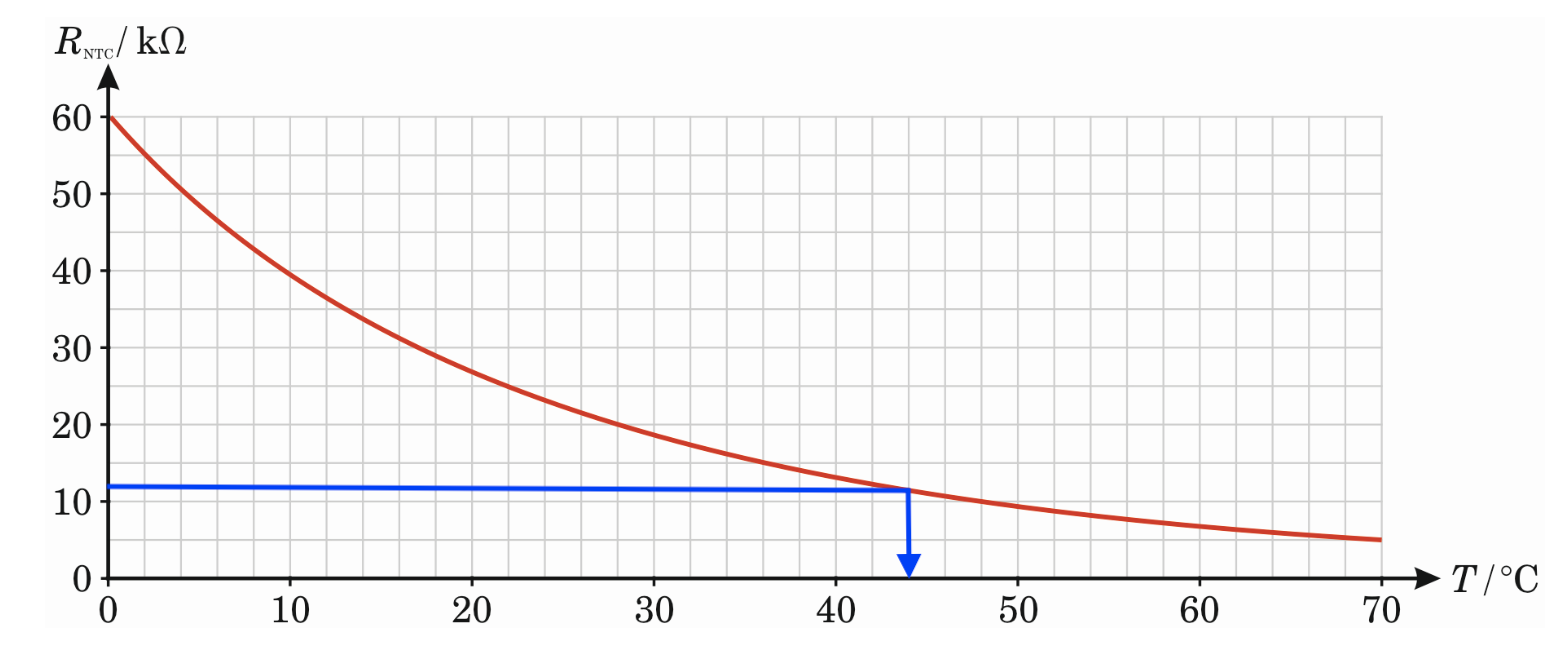
\includegraphics[width=0.8\textwidth]{TR.png}
\end{center}
\caption{Aflæsning på $(T, R _{\text{NTC} })$-grafen}
\label{fig:TR}
\end{figure}

\begin{question}{Lidar-sensor}{}
  En mobiltelefon udsender laserlys med frekvensen 3,19⋅1014 Hz i 500 ps.
\begin{itemize}
  \item[a.] Bestem antal svingninger i det udsendte laserlys.
\end{itemize}
Det udsendte laserlys reflekteres af en genstand og registreres af en sensor i mobiltelefonen. Telefonen beregner så afstanden til genstanden ved brug af lysets fart i luft og tiden fra lysets udsendelse til det registreres i telefonen.

Med henblik på at bestemme lysets fart i vand sender en mobiltelefon laserlys lodret ned i et bægerglas. Afstanden mellem telefonen og glassets bund er 40,0 cm. Der er 3,9 cm vand i bægerglasset. Telefonen måler afstanden 41,9 cm til glassets bund på trods af, at afstanden til glassets bund er 40,0 cm.
\begin{itemize}
  \item[b.] Bestem ved hjælp af målingerne en værdi for lysets fart i vand.
\end{itemize}
\end{question}
\sol \\
\textbf{a.}


\end{document}
